\chapter{PTMcosmos}
\label{chap:ptmcosmos}



\section{Summary}
PTMcosmos is a comprehensive database with an interactive web portal designed to catalog and visualize post-translational modifications (PTMs) in humans. It contains 469,183 experimentally-validated PTM sites and their supporting evidence from UniProt Knowledge Base, PhosphoSitePlus, and Clinical Proteomic Tumor Analysis Consortium (CPTAC). PTMcosmos summarizes the entire spectrum of CPTAC proteomics data on human cancer patients, including protein and PTM peptide abundance data from 10 different cancer types. Additionally, PTMcosmos contains cancer somatic mutations from the Cancer Genome Atlas (TCGA), thus allowing for the collective integration and analysis of different data types.  In PTMcosmos, we have built an ensemble of interactive visualization tools that will allow researchers to investigate altered PTM functions due to genetic alterations in close proximity. The database is live at \url{https://ptmcosmos.wustl.edu}. Furthermore, we used PTMcosmos to investigate PTM regulation across cancer types. First, we investigated the differential abundance of the PTM sites of cancer driver genes, focusing primarily on phosphorylation of the tumor suppressor retinoblastoma protein (encoded by \gene{RB1})  and acetylation of the histone acetyltransferase E1A Binding Protein P300 (\gene{EP300}) across cancer types. We analyzed the association between these PTM events and downstream targets, as well as with tumor subtypes, significantly mutated gene (SMG) mutation status  and clinical features. Second, we investigated the association of the protein abundance of cancer driver genes with ubiquitylsites in lung squamous cell carcinoma (LSCC) to nominate potentially novel modes of regulation of these proteins’ activity. We further analyzed the tumor subtype specificity and tumor-normal abundance changes of these ubiquitylsites and their corresponding substrate proteins, identifying several EGFR ubiquitylsites which may regulate EGFR abundance in LSCC. Finally, we identified the linear and spatial clustering of mutations and PTM sites, identifying multiple mutation-PTM clusters in cancer related genes, including TP53, PIK3CA, CTNNB1, EGFR, and IDH1. We envision that PTMcosmos will serve both the CPTAC consortium and the wider research community to better understand the role of PTMs in cancer.


\section{Introduction}



\section{Results}


\begin{figure}[tb]
    \centering
    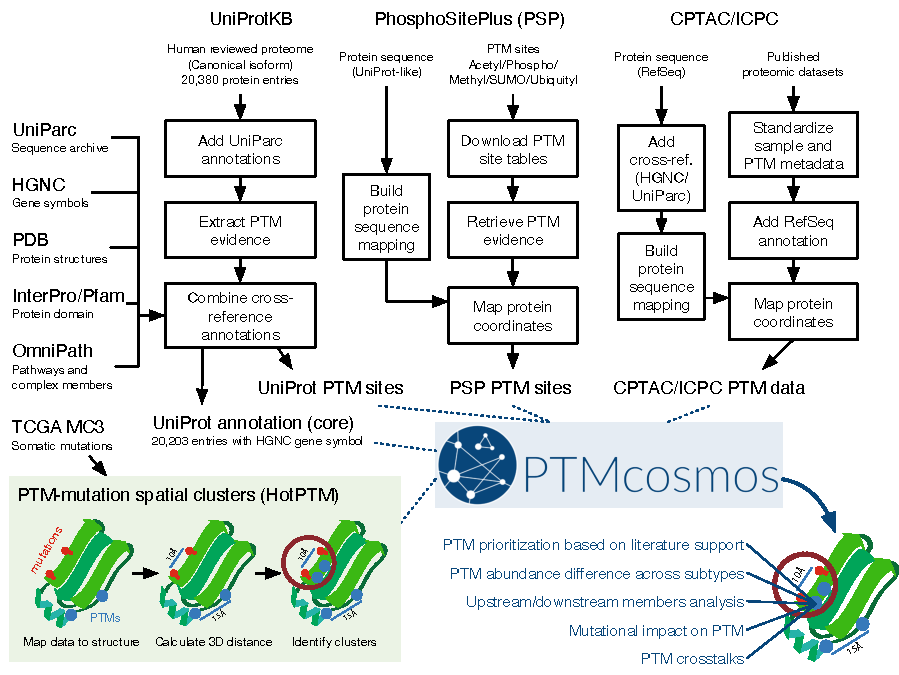
\includegraphics[width=0.9\linewidth]{figures/chap03_ptmcosmos/figure1_ptmcosmos_workflow.pdf}
    \caption[PTMcosmos overview.]{PTMcosmos overview.}
    \label{fig:ptmcosmos-workflow}
\end{figure}

\begin{figure}[tbp]
    \centering
    \phantomlabel{fig:ptmcosmos-stats-by-cancer}
    \phantomlabel{fig:ptmcosmos-stats-publications-per-ptm}
    \phantomlabel{fig:ptmcosmos-stats-publications-per-year}
    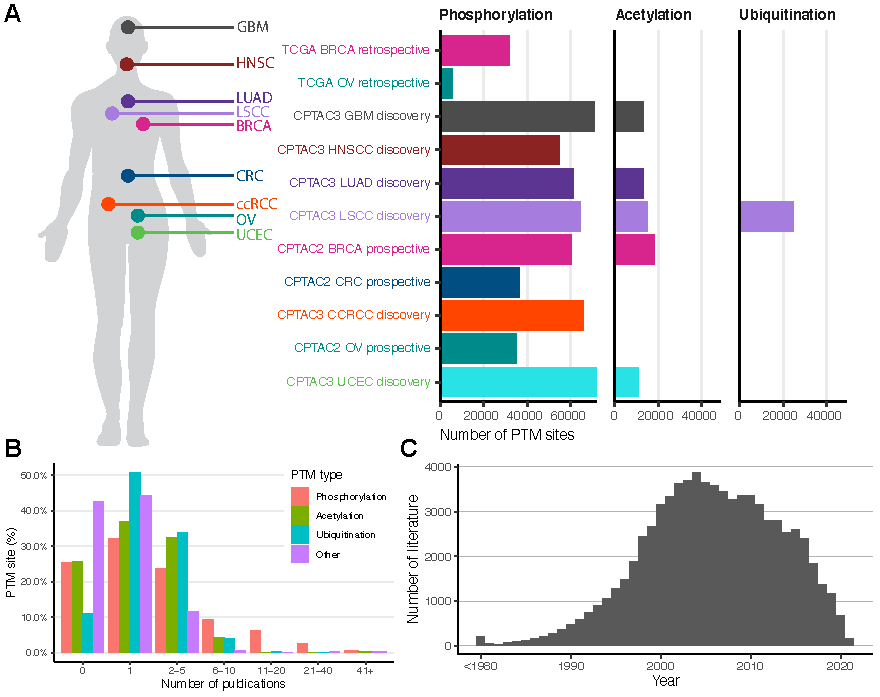
\includegraphics[width=\linewidth]{figures/chap03_ptmcosmos/figure1_ptmcosmos_stats.pdf}
    \caption[Supporting details of the mutation comparison.]{%
        Supporting details of the mutation comparison.
        \subref{fig:ptmcosmos-stats-by-cancer}
        \subref{fig:ptmcosmos-stats-publications-per-ptm}
        \subref{fig:ptmcosmos-stats-publications-per-year}
    }
    \label{fig:ptmcosmos-stats}
\end{figure}


\begin{figure}[tbp]
    \centering
    \phantomlabel{fig:ptmcosmos-map-stats-schematic}
    \phantomlabel{fig:ptmcosmos-map-stats-acetyl}
    \phantomlabel{fig:ptmcosmos-map-stats-ubiquityl}
    \phantomlabel{fig:ptmcosmos-map-stats-phospho}
    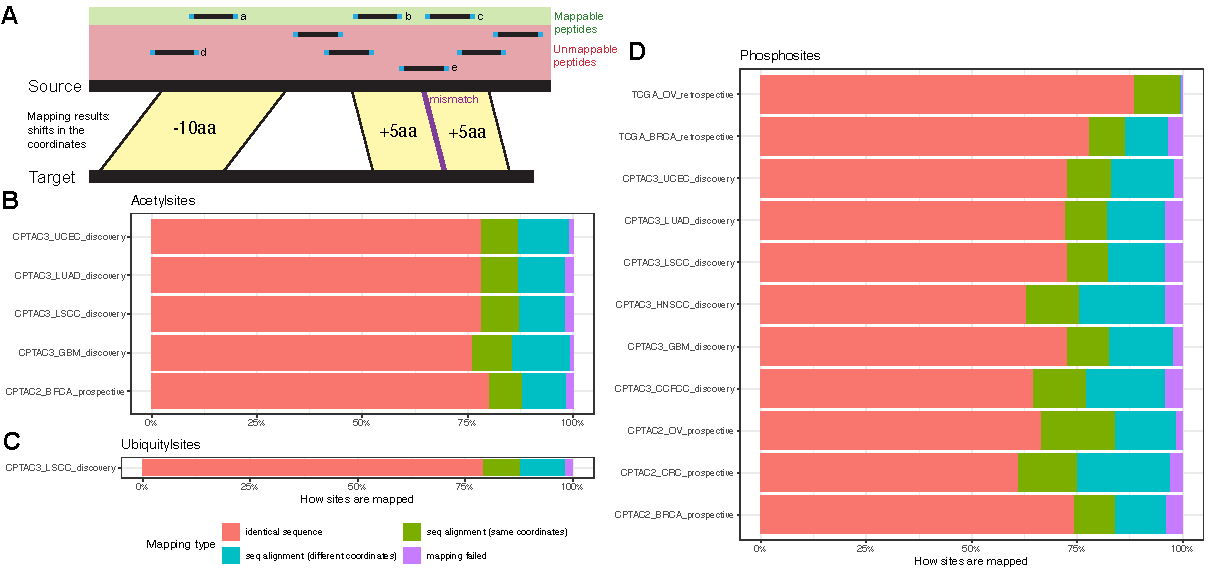
\includegraphics[width=\linewidth]{figures/chap03_ptmcosmos/figures1_mapping_stats.pdf}
    \caption[Supporting details of the peptide re-annotation and coordinate mapping.]{%
        Supporting details of the peptide re-annotation and coordinate mapping.
        \subref{fig:ptmcosmos-map-stats-schematic}
        \subref{fig:ptmcosmos-map-stats-acetyl}
        \subref{fig:ptmcosmos-map-stats-ubiquityl}
        \subref{fig:ptmcosmos-map-stats-phospho}
    }
    \label{fig:ptmcosmos-map-stats}
\end{figure}

\begin{figure}[tbp]
    \centering
    \phantomlabel{fig:ptmcosmos-site-detail-venn}
    \phantomlabel{fig:ptmcosmos-site-detail-pathway-domain}
    \phantomlabel{fig:ptmcosmos-site-detail-phspho-tyr}
    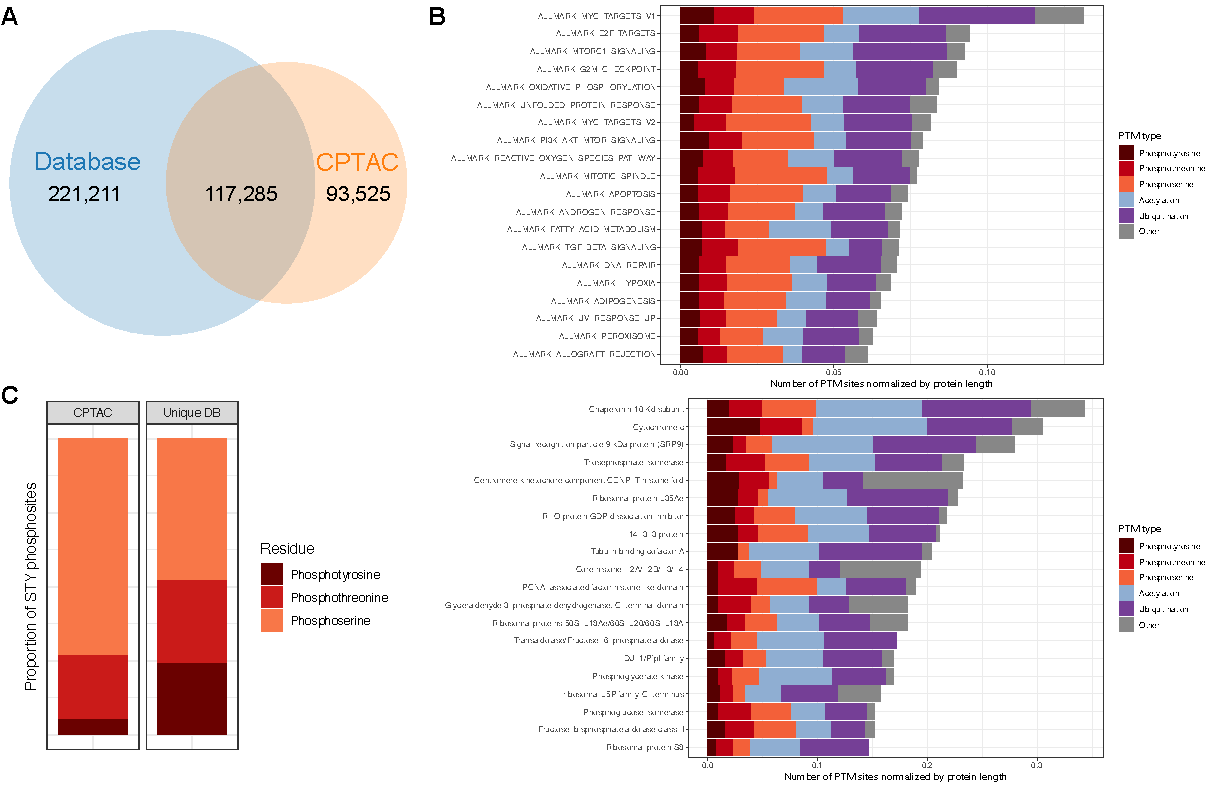
\includegraphics[width=\linewidth]{figures/chap03_ptmcosmos/figure2_ptmcosmos_site_detail.pdf}
    \caption[Descriptive analysis of the PTM sites in PTMcosmos.]{%
        Descriptive analysis of the PTM sites in PTMcosmos.
        \subref{fig:ptmcosmos-site-detail-venn}
        Venn diagram showing unique DB/CPTAC sites.
        \subref{fig:ptmcosmos-site-detail-pathway-domain}
        The top Hallmark pathways and PFAM domains (Y axis) represented among all PTM sites in PTMcosmos. For each pathway or domain, the number of PTM sites (X axis) is normalized by the total protein sequence length of entries in the given pathway or domain.
        \subref{fig:ptmcosmos-site-detail-phspho-tyr}
        The proportion of tyrosine phosphosites present among all CPTAC sites compared to sites uniquely present in PhosphositePlus or UniProtKB (referred to as ``unique DB'' sites).
    }
    \label{fig:ptmcosmos-site-detail}
\end{figure}

\begin{figure}[tb]
    \centering
    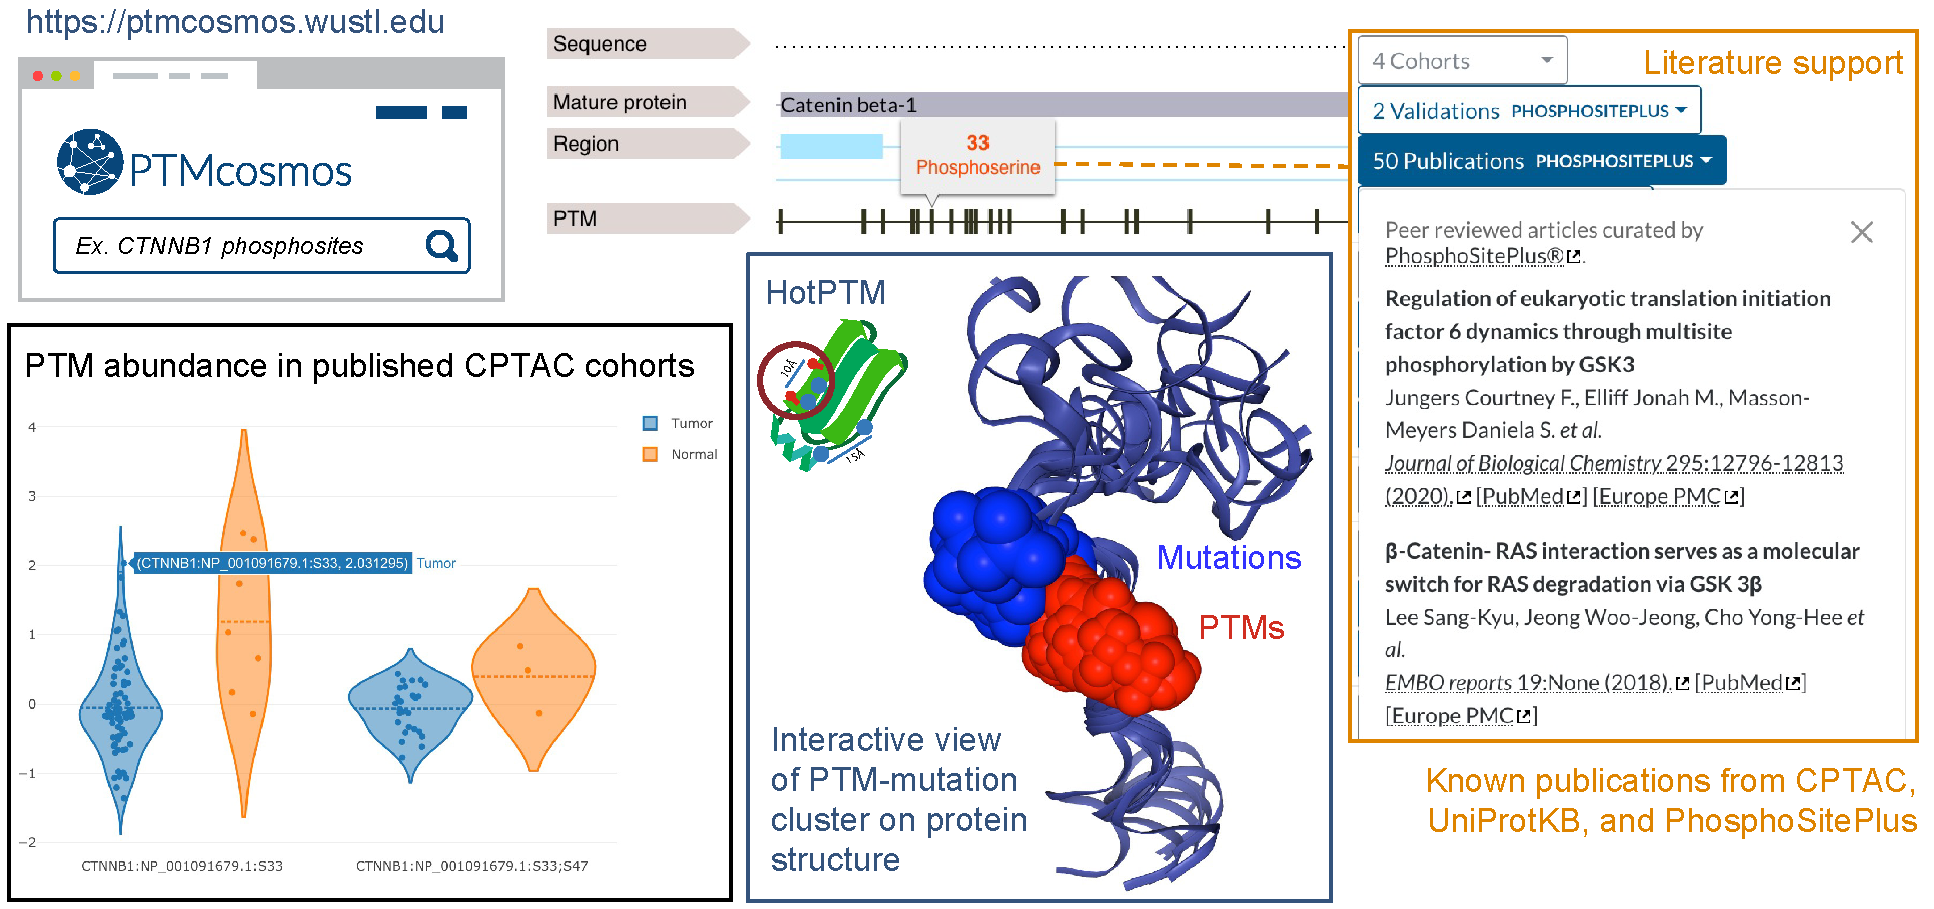
\includegraphics[width=\linewidth]{figures/chap03_ptmcosmos/figure3_ptmcosmos_usage.pdf}
    \caption[PTMcosmos usage demonstration.]{%
        PTMcosmos usage demonstration using β catenin phosphosites as an example. From right to left, the phosphosite S33, from the literature, is known to regulate the degradation of itself. The mutational impact analysis by HotPTM shows that endometrial cancer samples frequently harbor nearby mutations that disrupt this phosphosite. Finally, users can quickly check the relative abundance change at peptide level in every published CPTAC cohort.
    }
    \label{fig:ptmcosmos-usage-demo}
\end{figure}


\begin{figure}[p]
    \centering
    \phantomlabel{fig:ptmcosmos-de-overview}
    \phantomlabel{fig:ptmcosmos-ep300-prot-paint}
    \phantomlabel{fig:ptmcosmos-ep300-hist-acetyl}
    \phantomlabel{fig:ptmcosmos-ep300-assoc}
    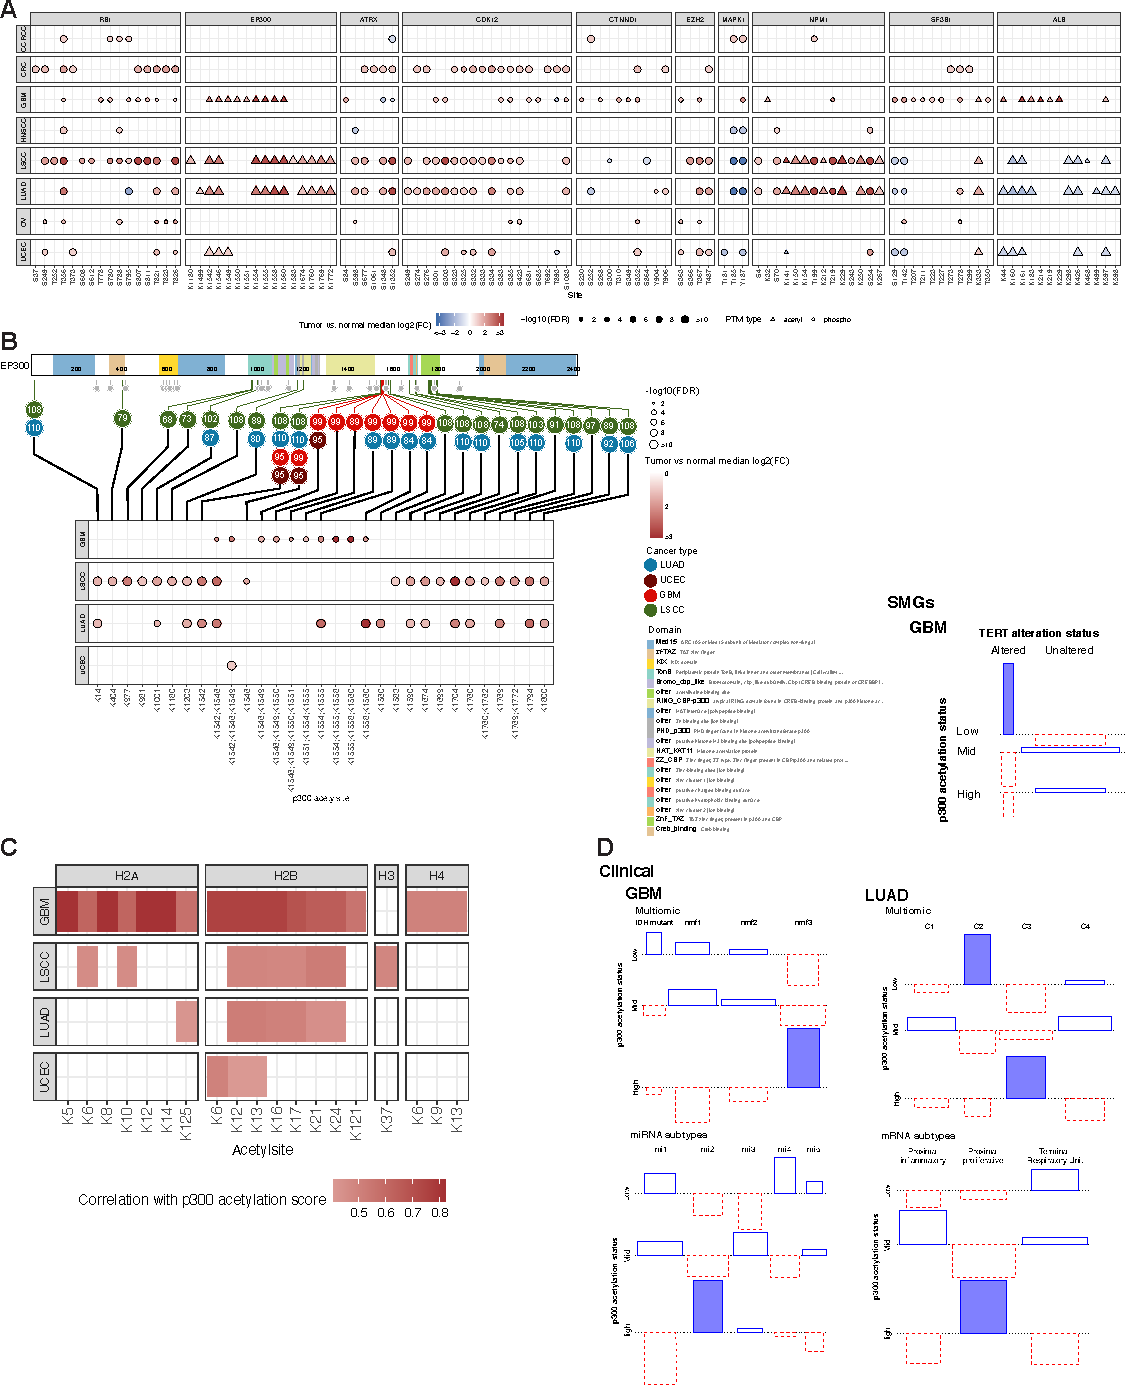
\includegraphics[width=\linewidth]{figures/chap03_ptmcosmos/figure4_ptmcosmos_ep300.pdf}
    \caption[Differential expression analysis of sites in PTMcosmos.]{%
        Differential expression analysis of sites in PTMcosmos.
        \subref{fig:ptmcosmos-de-overview}
        Overview of differentially expressed driver gene acetyl- and phosphosites across 8 cancer types.
        \legendcontdnote
    }
    \label{fig:ptmcosmos-ep300}
\end{figure}
\begin{figure}[t]
    \centering
    \legend{%
        \legendcontdref{fig:ptmcosmos-ep300}
        \subref{fig:ptmcosmos-ep300-prot-paint}
        Differentially expressed acetylsites of the acetyltransferase p300 mapped onto the protein's domain structure. The numbers shown in the circles represent the number of samples in a cohort detecting the given acetylsite.
        \subref{fig:ptmcosmos-ep300-hist-acetyl}
        Heatmap showing the significant Pearson correlations between the aggregate p300 acetylation score and histone acetylsites.
        \subref{fig:ptmcosmos-ep300-assoc}
        Mosaic plot showing the associations between p300 acetylation status and categorical variables such as tumor subtypes and the alteration status of significantly mutated genes.
    }
\end{figure}


\begin{figure}[p]
    \centering
    \phantomlabel{fig:ptmcosmos-rb1-prot-paint}
    \phantomlabel{fig:ptmcosmos-rb1-e2f}
    \phantomlabel{fig:ptmcosmos-lscc-ubiquityl}
    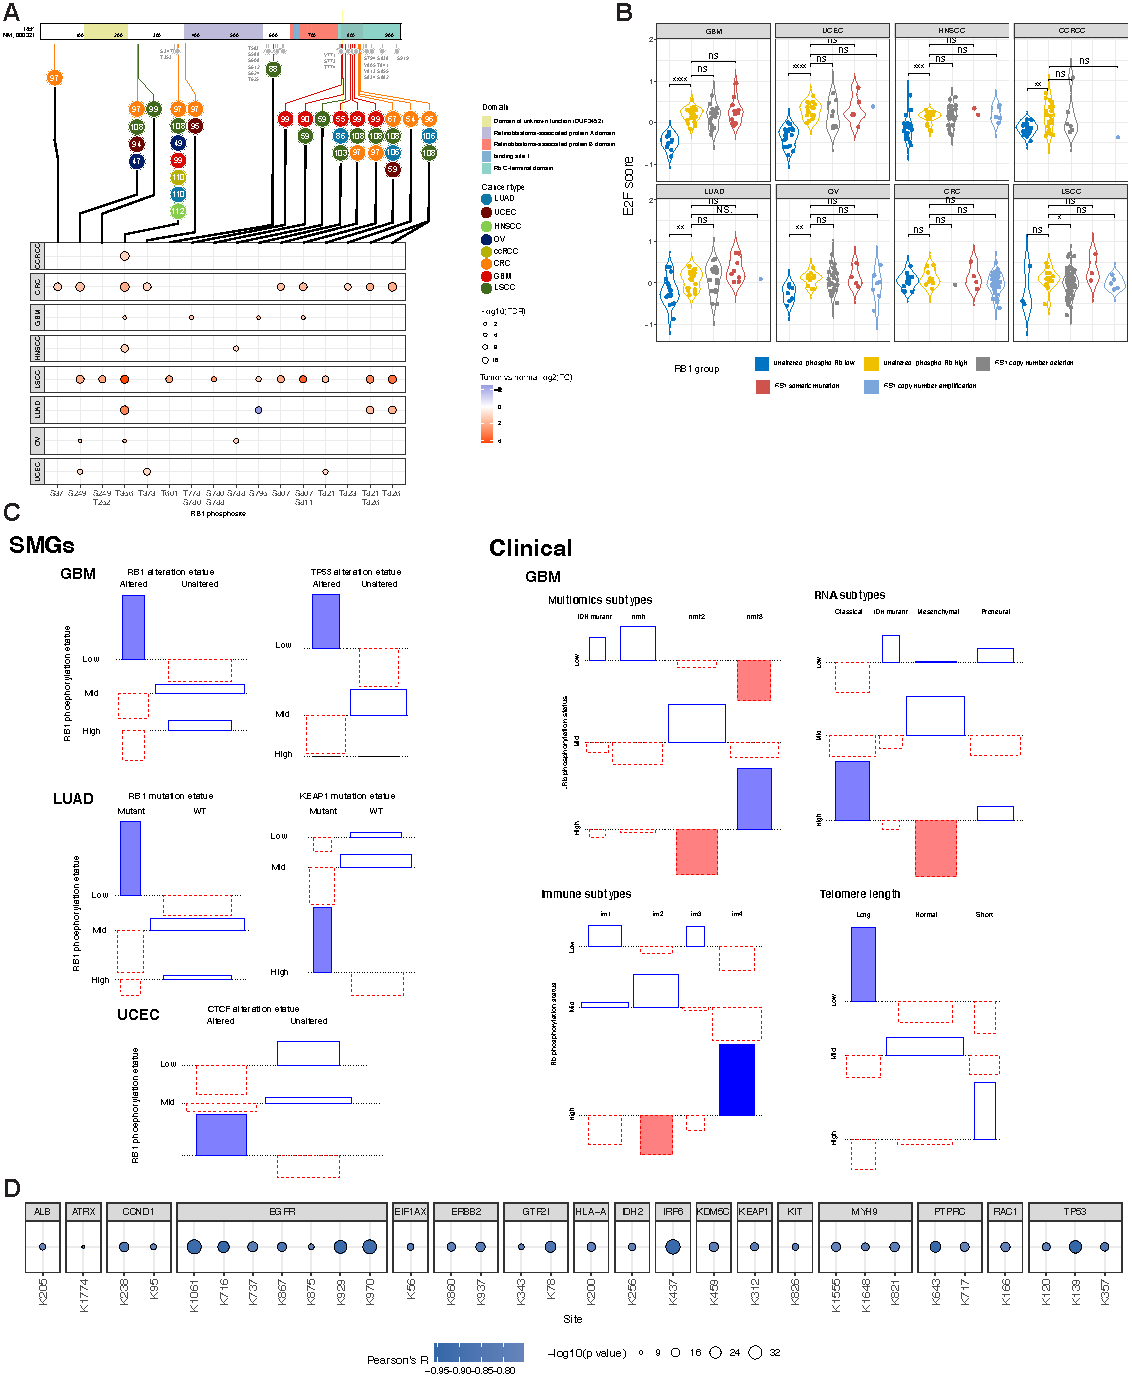
\includegraphics[width=\linewidth]{figures/chap03_ptmcosmos/figure5_ptmcosmos_rb1.pdf}
    \caption[Pan-cancer Rb phosphorylation analysis and LSCC ubiquitination analysis.]{%
        Pan-cancer Rb phosphorylation analysis and LSCC ubiquitination analysis.
        \legendcontdnote
    }
    \label{fig:ptmcosmos-rb1}
\end{figure}
\begin{figure}[t]
    \centering
    \legend{%
        \legendcontdref{fig:ptmcosmos-rb1}
        \subref{fig:ptmcosmos-rb1-prot-paint}
        Overview of differentially expressed Rb phosphosites across 8 cancer types and the mapping of these phosphosites onto the domain structure of Rb. The numbers shown in circles represent the number of samples in the given cohort detecting a phosphosite.
        \subref{fig:ptmcosmos-rb1-e2f}
        Averaged expression of E2F target genes (``E2F score'') stratified by RB1 alteration status or Rb phosphorylation status.
        \subref{fig:ptmcosmos-lscc-ubiquityl}
        Correlation in lung squamous cell carcinoma between normalized ubiquitylsite abundance and cognate protein abundance for cancer driver genes.
    }
\end{figure}


\begin{figure}[p]
    \centering
    \phantomlabel{fig:ptmcosmos-hotptm-enrich}
    \phantomlabel{fig:ptmcosmos-hotptm-structure}
    \phantomlabel{fig:ptmcosmos-hotptm-structure-complex}
    \phantomlabel{fig:ptmcosmos-hotptm-pi3k}
    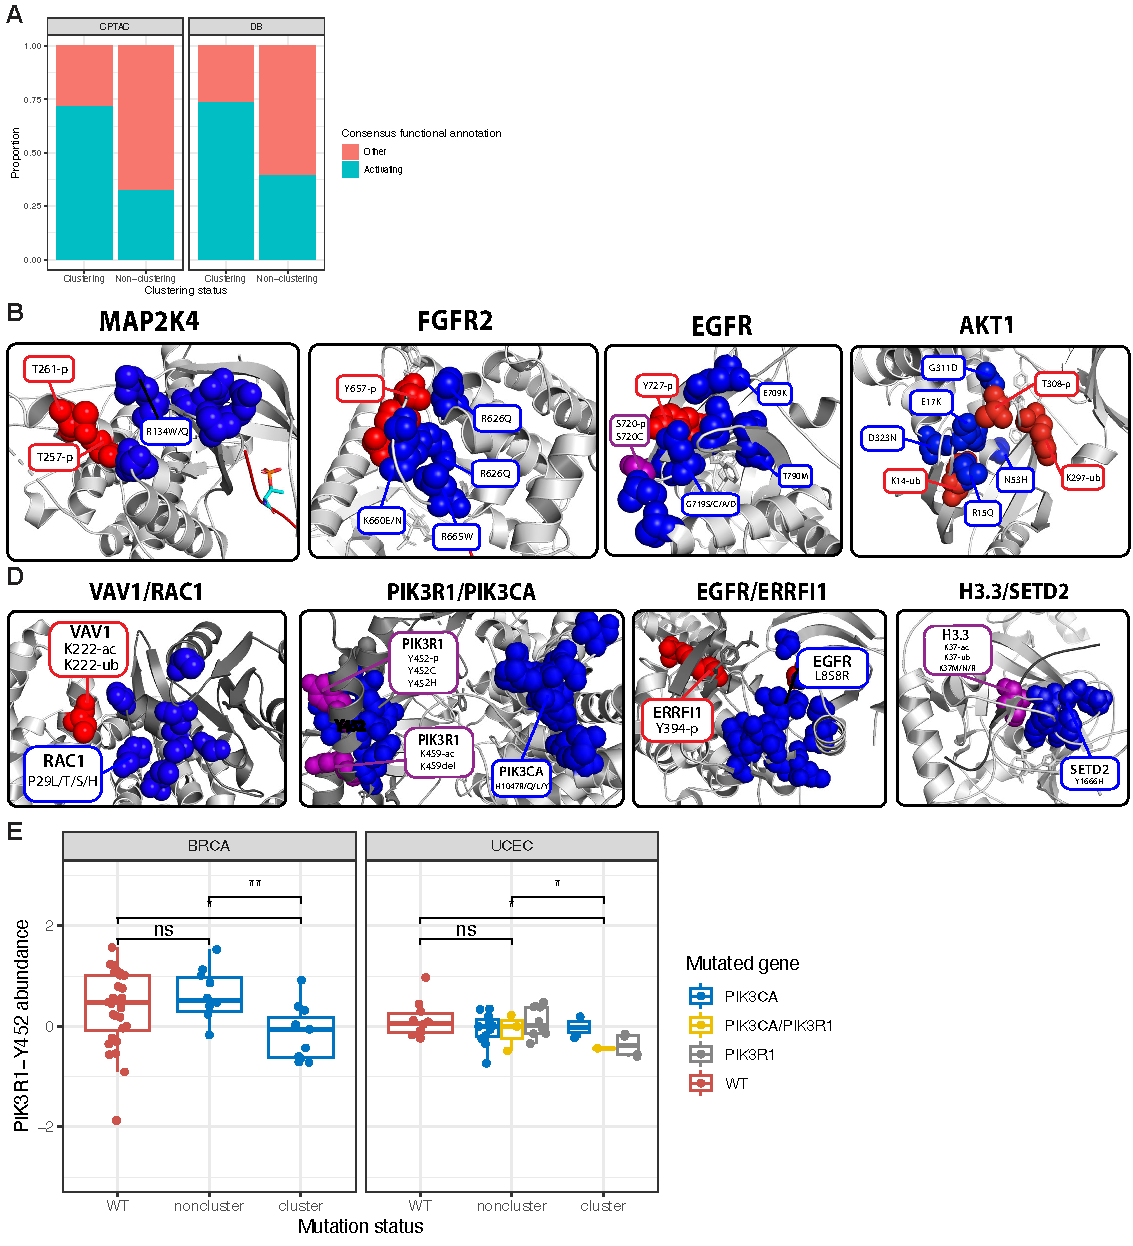
\includegraphics[width=\linewidth]{figures/chap03_ptmcosmos/figure6_ptmcosmos_hotptm.pdf}
    \caption[Spatial co-clustering of mutations and PTMs.]{%
        Spatial co-clustering of mutations and PTMs.
        \legendcontdnote
    }
    \label{fig:ptmcosmos-hotptm}
\end{figure}
\begin{figure}[t]
    \centering
    \legend{%
        \legendcontdref{fig:ptmcosmos-hotptm}
        \subref{fig:ptmcosmos-hotptm-enrich}
        Enrichment of activating mutations among mutations co-clustering with PTMs.
        \subref{fig:ptmcosmos-hotptm-structure}
        Selected mutation-PTM clusters mapped onto crystal structures obtained from the Protein Data Bank. Red spheres represent the residues modified by PTM sites, while blue spheres represent the residues affected by mutations.
        \subref{fig:ptmcosmos-hotptm-structure-complex}
        Visualization of mutation-PTM clusters spanning protein complexes. Purple spheres represent residues affected by both PTM sites and mutations.
        \subref{fig:ptmcosmos-hotptm-pi3k}
        Relative abundance of the PIK3R1-Y452 phosphosite in BRCA and UCEC stratified by mutation co-clustering status.
    }
\end{figure}

\section{Discussion}



\section{Methods}

\subsection{CPTAC proteomic data processing}

\tref{tab:ptmcosmos-peptide-db} \url{https://github.com/ccwang002/cptac_proteome_preprocess}


\begin{table}[tbp]
    \centering
    \caption{CPTAC peptide search databases used by different disease working group.}
    \label{tab:ptmcosmos-peptide-db}
    \begin{threeparttable}[b]
    \begin{tabular}{@{}llll@{}}
    \toprule
    Phase & Cohort & Database & Notes \\
    \midrule
    \multirow{2}{*}{\begin{tabular}[c]{@{}l@{}}CPTAC2/TCGA\\ retrospective\end{tabular}}
        & BRCA  & RefSeq 20130727   & Broad Institute \\
        & OV    & RefSeq 20111201   & PNNL \\
    \midrule
    \multirow{3}{*}{\begin{tabular}[c]{@{}l@{}}CPTAC2\\ prospective\end{tabular}}
        & OV    & CDAP (Refseq 2016)    & PNNL \\
        & CRC   & RefSeq 20171003\tnote{*}  & Use RefSeq 2018 instead \\
        & BRCA  & CDAP (Refseq 2016)    & Broad Institute \\
    \midrule
    \multirow{8}{*}{\begin{tabular}[c]{@{}l@{}}CPTAC3\\ discovery\end{tabular}}
        & CCRCC & CDAP (Refseq 2018) & UMich \\
        & GBM   & CDAP (Refseq 2018) & PNNL \\
        & HNSCC & CDAP (Refseq 2018) & UMich \\
        & LUAD  & CDAP (Refseq 2018)\tnote{\textdagger} & Broad Institute \\
        & LSCC  & CDAP (Refseq 2018)\tnote{\textdagger} & Broad Institute \\
        & PBTA  & CDAP (Refseq 2018) & MS3 spectra \\
        & PDAC  & CDAP (Refseq 2018) & UMich \\
        & UCEC  & CDAP (Refseq 2018) & PNNL \\
    \bottomrule
    \end{tabular}
    \begin{tablenotes}
    \item [*] Database uses hg38 genome reference.
    \item [\textdagger] Database includes smORFs.
    \end{tablenotes}
    \end{threeparttable}
\end{table}


\subsubsection{Harmonize Coordinate}
Only considered the canonical reviewed UniProt entries 
If the identical protein sequence can be found, mapped to them directly
Otherwise, perform global protein sequence alignment
To the UniProt entry of the same gene
Create coordinate segments of consecutive matches (don't allow any amino acid mismatch)
Only mapped the site when a full peptide (plus the 1 additional flanking aa) is in the coordinate segment

